\section{Design and Approach}

AUTOSAR provides a standardization of the software stacks that are employed in Automotive systems. It allows collaboration between various partners by standardization of the data exchange format and integration of basic software and application software from various partners on a single ECU via a middleware and across the vehicle network.
AUTOSAR supports broad variety of domains which includes but not limited to:
\begin{itemize}
	\item body/comfort.
	\item driver assistant systems.
	\item powertrain.
	\item chassis control.
	\item occupation and pedestrian safety.
\end{itemize}

\section{OS Internals}

AUTOSAR extends OSEK/VDX Operating systems standards which finds wide adoption in automotive systems.
OSEK OS is an event triggered operating system. This provides high flexibility in the design and maintenance of the system. Event triggering gives freedom of selecting from a wide range of events to drive scheduling at runtime and this includes angular rotation, local timer , global time source, error events etc.
\subsection{BSW Scheduler}
BSW Scheduler provides the basic abstraction for handling of task behavior specific to the timing and control.
AUTOSAR Specification neither provides nor recommends any specific implementation of the BSW Scheduler but specifies the feature set that are to be provided.
BSW Scheduler is not a competing entity to AUTOSAR OS Scheduler, instead it provides following features:
\begin{itemize}
	\item embed BSW modules in AUTOSAR Context.
	\item trigger main processing functions of the BSW Module.
	\item Apply data consistency mechanism for the BSW modules(e.g. Locking mechanisms.)
\end{itemize}
For example, BSW Module provides EnableAllInterrupts and DisableAllInterrupts APIs as a meaning of serializing the execution of the critical sections.
The BSW scheduler files encompasses a SchM.h file providing the abstraction to start the task corresponding to the BSW Scheduler and set of support file which are of the form BSW\_<Module Prefix>.h.
The module specific files are a form of contract to support the data consistency mechanism promised by the BSW Scheduler.
\begin{figure}[h]
	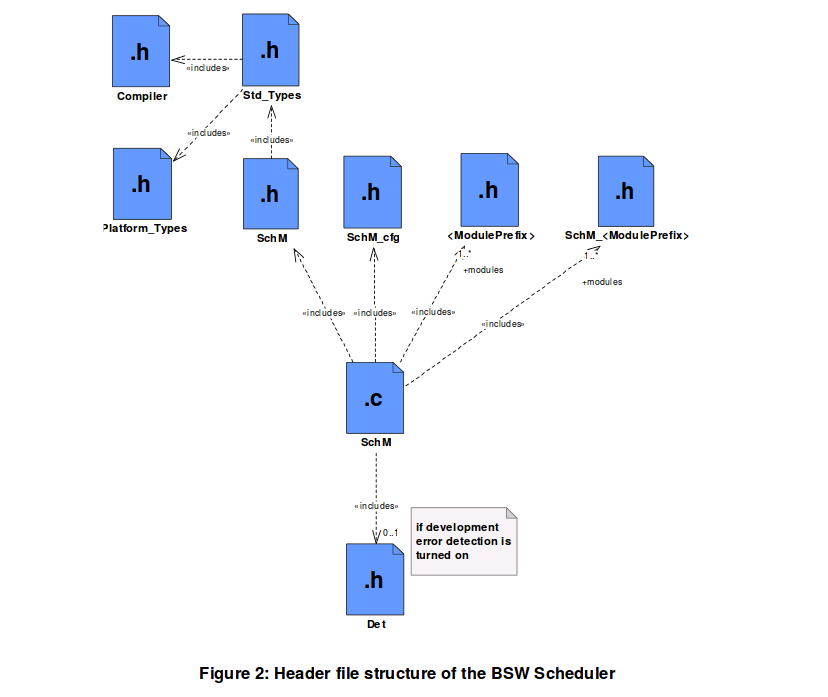
\includegraphics[scale = 0.5]{Pictures/BSW_Schduler.png}
\end{figure}
BSW Scheduler can be implemented as a task that will handle read write operations.
BSW Scheduler cannot invoke the main functions that can enter the wait state.
Thus BSW Scheduler handler the entities, which being the individual actions that can be handled in the context of a task, while the task level control resides with AUTOSAR OS Scheduler.
\subsection{OS Interrupts}
Interrupts under AUTOSAR are classified into cat1 and cat2.
The difference between the two are as follows:
\begin{itemize}
	\item cat1 interrupts are not allowed to make OS calls. The only APIs they can call are to enable and disable interrupts. While cat2 interrupts can call most OS calls, while others are illegal.
	\item cat1 interrupts have lower latency than cat2.
	\item There exists no support for cat1 interrupts from OS, to abstract the interrupt and its handler from the hardware in portable way and is depends on the platform and the tool-chain.
	\item In cat1 interrupt handler there is no need to lock the critical region as it will be shared with task or interrupt of lower priority.
\end{itemize}
Initialization steps for the interrupt handler involves defining vector table and correct entry for handler function.
cat2 interrupt uses ISR macro to define the interrupt handler, advantage of this being, it encapsulates the handler function.
Mutual exclusion in cat2 interrupts are provided by BSW Scheduler in the for of disabling and enabling interrupt sub group.
In case of cat1 interrupts if the mutual exclusion is required, it can be done in terms of disabling all the interrupts. As this seriously affects the overall performance of the system, cat1 region should be kept to minimum.
\subsection{Time Service Module}
Time Service Module is part of the service layer and provides following features:
\begin{itemize}
	\item Time measurement.
	\item Time based state machine.
	\item Timeout supervision
	\item Busy Loop feature.
\end{itemize}
Time Service Module does not sit on top of the timer stack and does not use and provide all the features of GPT Driver.

\subsection{Time Base Manager}
Synchronized time base manager provides APIs to its customers or time bases, which are synchronized with other time bases of the distributed systems, thus acting as a time broker.
Time Base Manager acts as the central module to which provides absolute time of the system. Typical use case include Sensor fusion(Temporal correlation various sensor data.), Event data recording(Temporal correlation of the logs while reporting on system crash or on detection of an anomaly), and diagnostic event storage.
The customers to the Time Base Manager can be triggered or active. AUTOSAR OS is currently supported as a triggered customer.
A Global time network consists of atleast one Time master and atleast one Time Slave. \\
Figure below shows a representation of such a global time network.

\noindent%
\begin{minipage}{\linewidth}% to keep image and caption on one page
	\makebox[\linewidth]{%        to center the image
		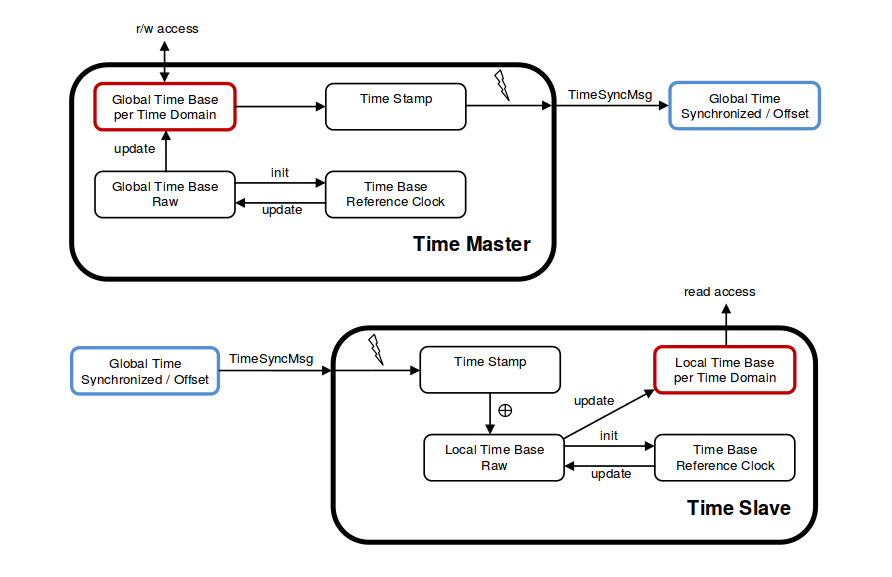
\includegraphics[keepaspectratio=true,scale=0.5]{Pictures/Global_Time_Base.png}}
\end{minipage}

Two different sets of time bases are provided. Time Domains 0-15 are synchronized time bases while Time Domains 16-31 are offset time bases.

\subsection{Core OS Specifications}
In AUTOSAR systems internal communication is provided by RTE or COM at least one of which will be present in the ECUs.
AUTOSAR OS thus when used in an AUTOSAR system does not need to support communication.
One of the key component AUTOSAR OS extends on OSEK/VDX is Schedule tables.
In OSEK it is possible to provide statically defined activation mechanism using an OSEK counter and alarms. To provide runtime modification of the activation, it is necessary to maintain synchronization between the alarms.
Schedule table provides a solution to this issue of synchronization by providing an encapsulation to the statically defined expiry point.
In a schedule table an expiry point corresponds to one or more actions that should occur in the system and corresponds to a fixed offset from the beginning of a schedule table.
Each schedule table is defined by a set of ticks and the os module will iterate over the ticks and invoke appropriate actions at expiry points. \\Figure below shows an example of schedule table.\\
\noindent%
\begin{minipage}{\linewidth}% to keep image and caption on one page
	\makebox[\linewidth]{%        to center the image
		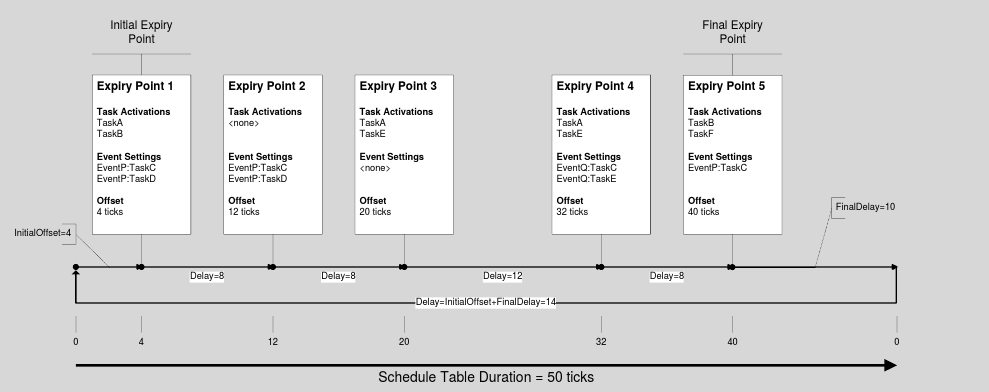
\includegraphics[keepaspectratio=true,scale=0.5]{Pictures/Schedule_Table.png}}
\end{minipage}


 
